
% Also note that the "draftcls" or "draftclsnofoot", not "draft", option
% should be used if it is desired that the figures are to be displayed in
% draft mode.
%
%\documentclass[draftcls, onecolumn]{IEEEtran}
\documentclass[conference, twocolumn]{IEEEtran}

%\usepackage[latin1]{inputenc} % Latin1
\usepackage[utf8]{inputenc} 	% UTF-8

%\usepackage{amsmath,amsthm}
\usepackage{amssymb}
%\usepackage{amsfonts}
\usepackage{bbm} % For indicator function
%\usepackage{breeq}
%\usepackage[pdftex]{graphicx}
\usepackage{graphicx}
\usepackage{color,psfrag}

% Dashed arrow and control the size of the braces due to underbrace
\usepackage{MnSymbol}
%\graphicspath{{./figures/}}

%Strike out the sentence
\usepackage[normalem]{ulem}

% Draw something blocks or ovelap
\usepackage{tikz}
\usepackage{siunitx}
\usepackage{cite} % Combining multiple citations


% New commands
\newcommand{\sub}[1]{_{\text{#1}}}

\newcommand{\pd}{\text{P}\sub{d}}
\newcommand{\pfa}{\text{P}\sub{fa}}

\newcommand{\pdd}{\bar{\text{P}}\sub{d}}
\newcommand{\prcvd}{P\sub{rcvd}}
\newcommand{\bprcvd}{\bar{P}\sub{rcvd}}

\DeclareMathOperator*{\maxi}{max}


%\DeclareGraphicsExtensions{.pdf}

%\iftwocolumn
	\newcommand{\figscale}{\columnwidth}
%\else
%	\newcommand{\figscale}{0.5\columnwidth}
%\fi

% Metadata
%\usepackage[final=true]{hyperref}
%\hypersetup{
%	pdfauthor = {Ankit Kaushik et al.},
%	pdftitle = {DySPAN 2015},
%	pdfsubject = {DySPAN 2015},
%	pdfcreator = {PDFLaTeX with hyperref package},
%	pdfproducer = {PDFLaTeX}
%	hidelinks = {true}
%}


% Used to break the theorems, proof between the columns
\allowdisplaybreaks

%used to equalize the last pages
%\usepackage{flushend}

\begin{document}
%
\title{Spectrum Sharing for 5G Wireless Systems}
\author{Ankit Kaushik, Felix Wunsch, Andrej Sagainov, Nicolas Cuervo, Johannes Demel, \\ Sebastian Koslowski, Holger Jäkel, Friedrich Jondral \\
Communications Engineering Lab, Karlsruhe Institute of Technology (KIT), Germany \\
{Ankit.Kaushik@kit.edu}}
\IEEEspecialpapernotice{(Spectrum Sharing Challenge)}
% make the title area
\maketitle
\thispagestyle{empty}
\pagestyle{empty}
\begin{abstract}
Understanding the performance of a spectrum sharing system by means of a hardware deployment is a challenging task. Motivated by this fact, we propose a prototype of a secondary system that co-exists with a primary system and simultaneously sustains the constraints defined by the regulatory. In this paper, we propose several key-techniques for the secondary system, which will be deployed on a hardware. 
\end{abstract}
\vspace{-3mm}
%%%%%%%%%%%%%%%%%%%%%%%%%%%%%%%%%%%%%%%%%%%%%%%%%%%%%%%%%%%%%%%%%%%%%%%%%%%%%%%%%%%%%%%%%
\section{Proposal} \label{sec:prop}
%%%%%%%%%%%%%%%%%%%%%%%%%%%%%%%%%%%%%%%%%%%%%%%%%%%%%%%%%%%%%%%%%%%%%%%%%%%%%%%%%%%%%%%%%
In order to render an optimum performance, we propose a cross-layer optimization of the Secondary User (SU) system. In this regard, corresponding to physical and medium access layer, we illustrate key-techniques envisioned for the challenge. More importantly, we briefly discuss the impact of these techniques on the performance of the system and consequently outline our proposed solution. 
\vspace{-3mm}
\subsection{Physical layer}
\subsubsection{SU Waveform}
The waveform design signifies the most fundamental aspect of the secondary system. A suitable waveform delivers a high spectral efficiency for the secondary system and low out-of-band emission, thereby causing minimum interference to the adjacent primary channels. Motivated by this fact, we employ Filter Bank Multi Carrier (FBMC) for the secondary transmission. In addition, we investigate the performance of FBMC against OFDM, in order to ensure that we exploit the benefits of FBMC over state-of-the-art waveform. 
\subsubsection{Sensing}
In spectrum sharing, protecting the primary receiver against interference is an absolute paramount. For detecting a primary signal, several detection techniques such as Energy Detection (ED), matched filtering and feature-based detection exist. Due to its versatility towards unknown primary signals, ED is widely investigated in the literature. In the view of this, we employ ED at the Secondary Transmitter (ST). 


Probability of detection ($\pd$) and probability of false alarm ($\pfa$) quantify the performance of the secondary system. From the regulatory perspective, $\pd$ is critical for the primary system because it precludes the ST from causing interference at the Primary Receiver (PR). In this regard, we propose a constant detection rate, according to which the ST sustains a minimum level $\pdd$ such that $\pd \ge \pdd$. According to \cite{Tan08}, threshold $\epsilon$ in correspondence to the ED is determined as 
\begin{equation} 
\epsilon = \bprcvd \left(\mathcal{Q}^{-1} (\pdd) \sqrt{\frac{2}{N}} + 1 \right), 
\end{equation} 
where $\mathcal{Q}^{-1}(\cdot)$ represents inverse Q-function \cite{grad}, $N$ is the number of samples used for sensing and $\bprcvd$ is the average power received at the ST from the Primary Transmitter (PT). In practice, to determine $\epsilon$, the knowledge of $\bprcvd$ is required. Hence, we acquire this knowledge during the learning phase of the challenge. 

However, with additional knowledge about the primary system, e.g., its frame structure (preamble sequence), we propose a feature-based detector as a secondary detector. This is done to improve the performance of our detector. 

\subsubsection{Beamforming}
With the existence of multiple antennas, we employ: i) receiver beamforming at the ST and, ii) receiver beamforming at the Secondary Receiver (SR). During the sensing period, the ST could steer its beam to improve the quality of the link between the PT and the ST, thereby increasing the received power from the PT. This would further enhance the detector performance. During data transmission, the SR would steer its beam towards the ST, this would improve the power received over the secondary link, thus, leading to an increase in the SU's throughput. Particularly at the SR, it is important to consider the interference from the PT. In this regard, we implement matched filtering to improve signal to noise ratio plus interference at the SR. Most importantly, the pre-factors required to perform transmitter and receiver beamforming are determined during the learning phase. %Moreover, based on the transmit beamforming can be extended to further improve the link quality  

\subsubsection{Antenna Diversity}
As a fallback solution to beamforming, we utilize antenna diversity at the ST that improves the performance of our detector. To accomplish this, we assume that the coherence time is larger than sensing duration and the antennas encounter independent fading. Each antenna undergoes a square law and integration operation of the primary signal resulting in energy samples $\{y_1, y_2,..., y_L\}$ from $L$ antennas. These energy samples go through either a combination ($y\sub{SLC} = \sum_{i=1}^L y_i$) or selection ($y\sub{SLS} = \maxi \{y_1, y_2,...,y_L \}$) process \cite{dig07}. 
%hence, termed as square law combiner and square law selector, respectively \cite{dig07}. 


\subsubsection{Time-Frequency Agility}
In addition to the performance of the detector, it is significant for the ST to utilize the available time-frequency gaps in the Primary User (PU) spectrum efficiently. Hence, it is reasonable to deploy a hardware that could scan the PU spectrum and simultaneously procure minimum latency. Here, latency signifies the interval between the detection of a time gap and start of SU transmission. This requirement can be proceeded with a hardware implementation (FPGA or ASIC). 
%To accomplish this, it is essential to realize these techniques using a hardware logic (ASIC or FPGA). 
However, most of the existing software defined architectures have either limited or no FPGA space available for incorporating sensing and the aforementioned techniques. In order to breakthrough this hardware bottleneck, we perform time-frequency agility by means of a software that scans a given channel (\SI{5}{MHz}) and allows hopping across the PU channels. With this, we employ sensing and proposed techniques for this channel. 
A hardware demonstration of such a system that performs sensing while hopping through the GSM downlink channels is presented in \cite{Kaushik13}. 
As an extension to existing software based methodology, we plan to port the proposed techniques, particularly the sensing, to FPGA.   


%\vspace{-2mm}
\subsection{Medium Access Layer}
\subsubsection{Learning}
Apart from the physical layer techniques, a further enhancement in the performance of the secondary system is procured by incorporating the learning process, whereby the ST captures the PU's medium access. In practice, the ST is required to select a single PU channel from the available channels and to perform sensing, followed by data transmission, once the selected channel is found idle. Hence, to utilize the time resources efficiently, it is important to optimize this selection process. In this regard, we apply static learning and reinforcement learning at the ST. 

According to static learning, the ST maintains a belief vector \cite{Zhao} $\Lambda = [u_1,..., u_i,...,u_N]$ for $N$ PU channels, where $u_i$ corresponds to the utilization probability for the $i^{\text{th}}$ channel. Now, the selection is in accordance to the utilization probabilities for each channel in the $\Lambda$, where $\Lambda$ is determined during the exploration/learning phase. The nomenclature static signifies that $\Lambda$ is never updated during the exploitation/optimization phase. Hence, the channel with least utilization probability is always the first channel selected for sensing. 

In contrast to static learning, subject to reinforcement learning, the ST updates $\Lambda$ during the exploitation phase. This update on $\Lambda$ is carried out by imposing a penalty when the selected channel $i$ is found busy. This penalty, added to the $u_i$, prevents the ST from selecting the penalized channel for a certain duration. This duration corresponds to the expected busy period of the penalized channel. %Hence, subject to reinforcement learning, the ST updates the $\Lambda$ during the exploitation phase. 
%\begin{figure}[!t]
%\centering
%\includegraphics[width = \columnwidth]{figures/Grafik_Poster}
%\label{fig:HW_gui}
%\end{figure}


%\vspace{-2mm}
%%%%%%%%%%%%%%%%%%%%%%%%%%%%%%%%%%%%%%%%%%%%%%%%%%%%%%%%%%%%%%%%%%%%%%%%%%%%%%%%%%%%%%%%%
\section{Proof-of-Concept} \label{sec:pof}
%%%%%%%%%%%%%%%%%%%%%%%%%%%%%%%%%%%%%%%%%%%%%%%%%%%%%%%%%%%%%%%%%%%%%%%%%%%%%%%%%%%%%%%%%
Here, we present the hardware feasibility of the techniques discussed in the previous section. In order to investigate the performance of the secondary system subject to the proposed techniques, a primary system compliant to IEEE 802.15 has been deployed, cf. \figurename~\ref{fig:SetUp}. The transmission based on FBMC and OFDM has been implemented, \figurename~\ref{fig:Waveform} illustrates a successful reception of the two waveforms at the SR. Finally, the performance of the learning algorithms has been depicted. \figurename~\ref{fig:Learning} illustrates the exploited opportunities in reference to the total opportunities generated in four PU channels, given the constraint that only a single PU channel from four channels is selected for sensing. To evaluate the performance of learning algorithms, an optimum strategy is considered, in which, once an opportunity is available in any of the four channels, it will be utilized by sensing the particular channel.
\begin{figure}[!t]
\centering
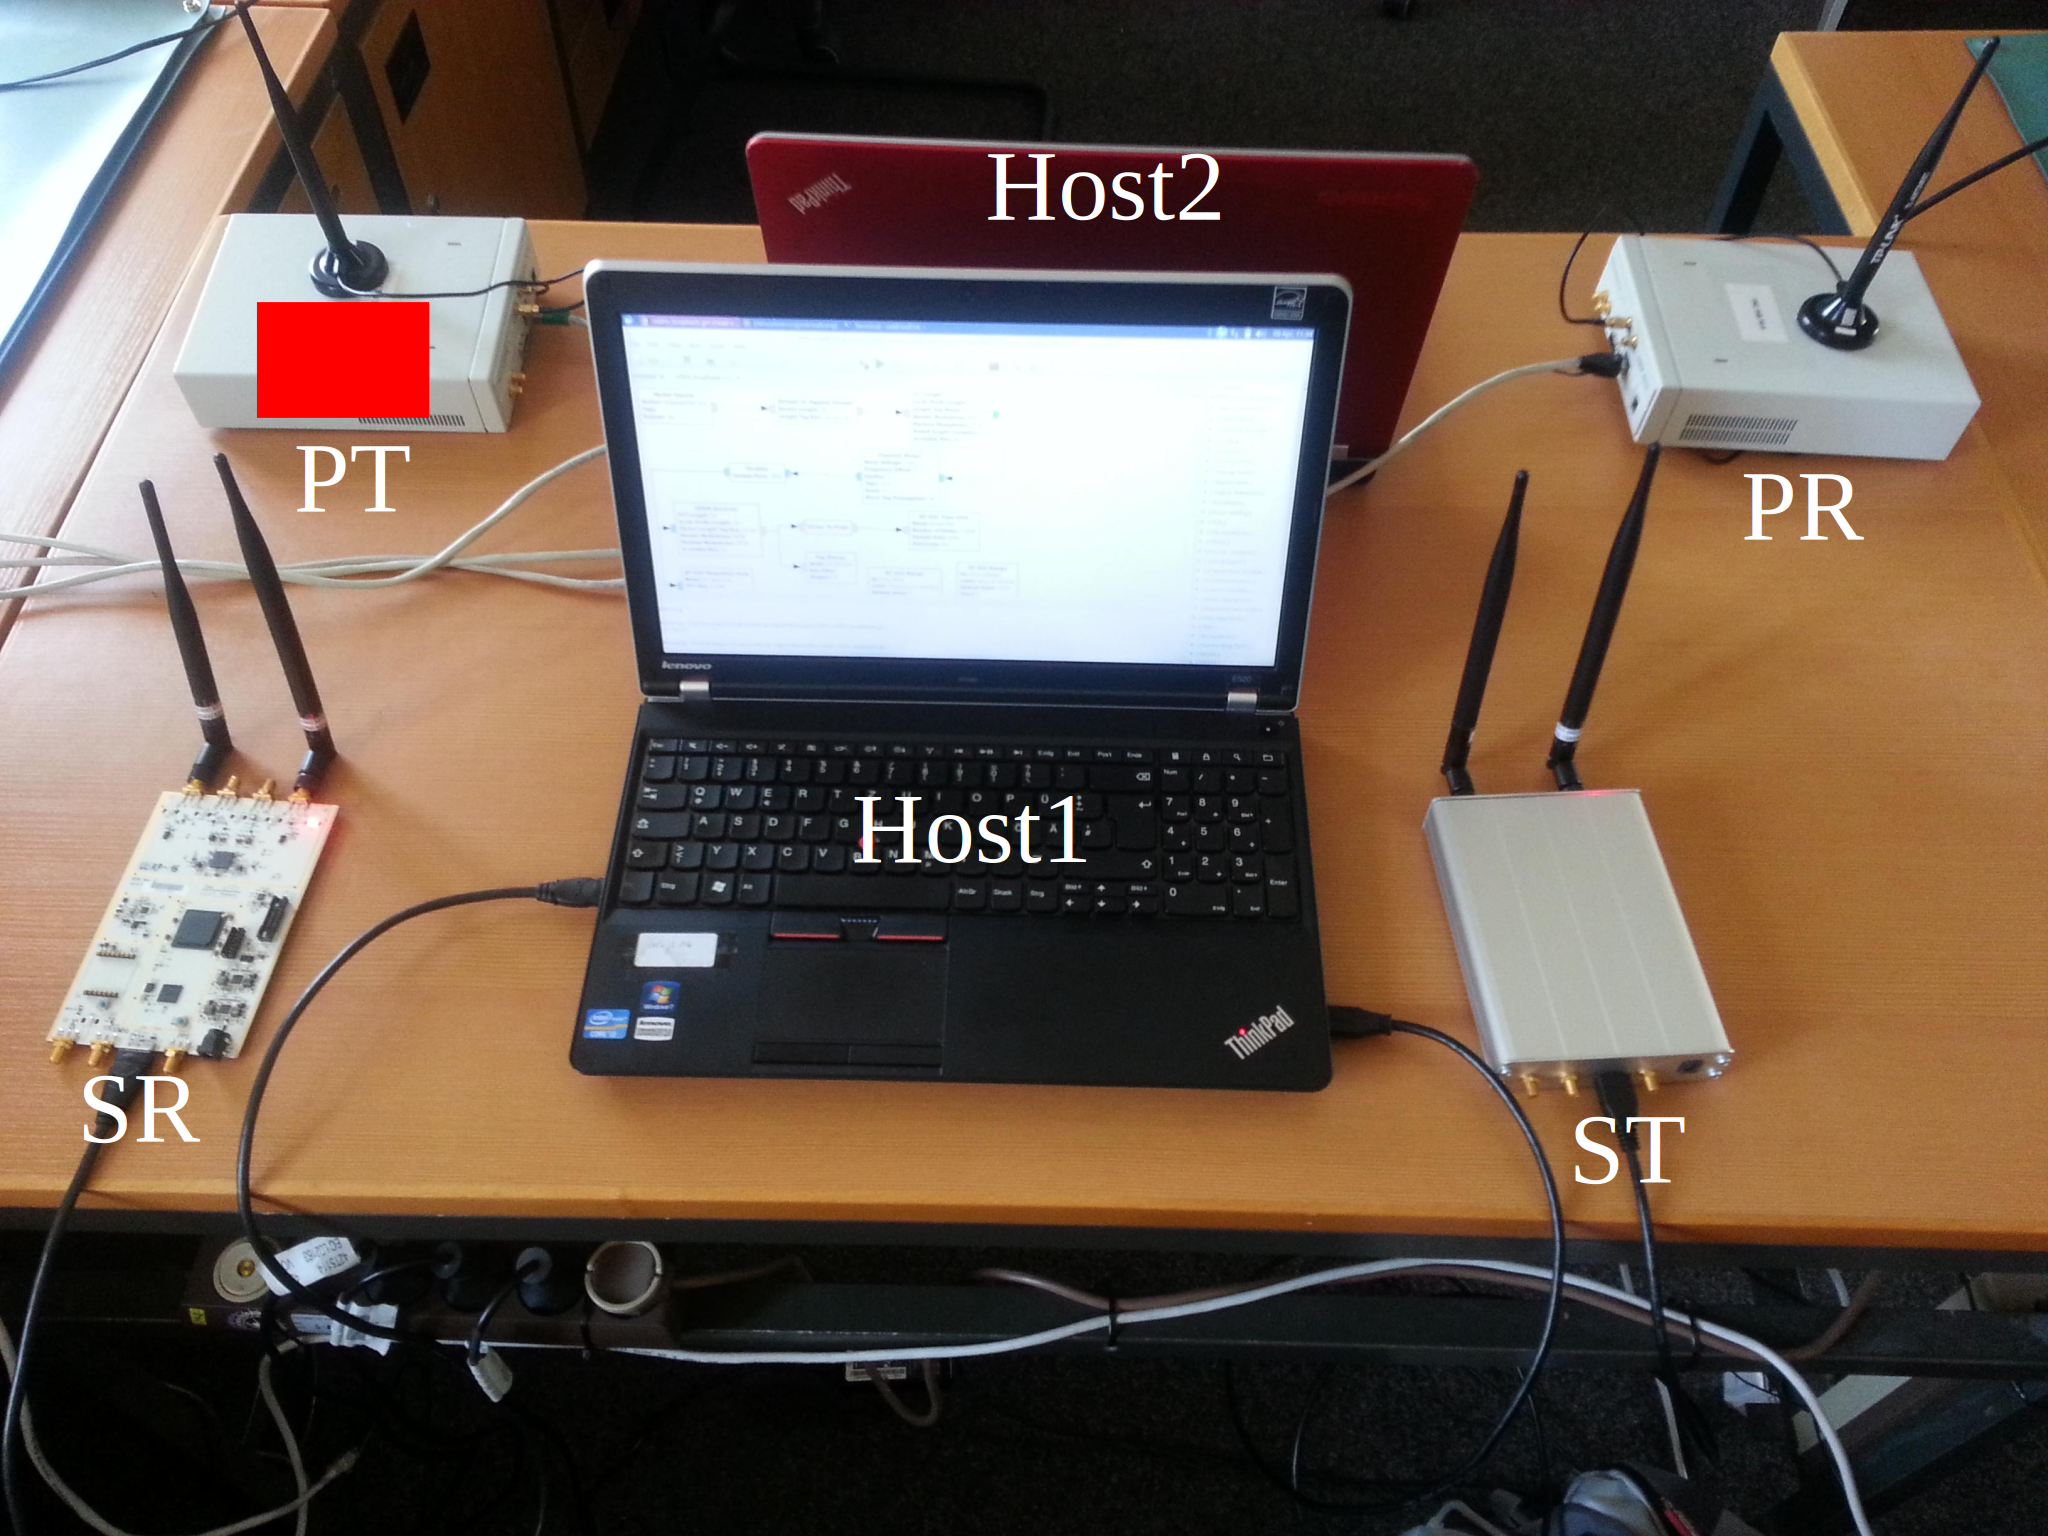
\includegraphics[width = 0.9 \columnwidth]{figures/SetUp}
\caption{Hardware setup demonstrating the primary and secondary system. The key-techniques mentioned in the paper are implemented on a software running on the host computers.} 
\vspace{-4mm}
\label{fig:SetUp}
\end{figure}
\begin{figure}[!t]
% This file is generated by the MATLAB m-file laprint.m. It can be included
% into LaTeX documents using the packages graphicx, color and psfrag.
% It is accompanied by a postscript file. A sample LaTeX file is:
%    \documentclass{article}\usepackage{graphicx,color,psfrag}
%    \begin{document}% This file is generated by the MATLAB m-file laprint.m. It can be included
% into LaTeX documents using the packages graphicx, color and psfrag.
% It is accompanied by a postscript file. A sample LaTeX file is:
%    \documentclass{article}\usepackage{graphicx,color,psfrag}
%    \begin{document}% This file is generated by the MATLAB m-file laprint.m. It can be included
% into LaTeX documents using the packages graphicx, color and psfrag.
% It is accompanied by a postscript file. A sample LaTeX file is:
%    \documentclass{article}\usepackage{graphicx,color,psfrag}
%    \begin{document}\input{OFDMvsFBMC}\end{document}
% See http://www.mathworks.de/matlabcentral/fileexchange/loadFile.do?objectId=4638
% for recent versions of laprint.m.
%
% created by:           LaPrint version 3.16 (13.9.2004)
% created on:           28-Apr-2015 10:28:34
% eps bounding box:     16 cm x 12 cm
% comment:              
%
%\begin{psfrags}%
%\psfragscanon%
%
% text strings:
\psfrag{s05}[t][t]{\fontsize{9}{13.5}\fontseries{m}\mathversion{normal}\fontshape{n}\selectfont \color[rgb]{0.15,0.15,0.15}\setlength{\tabcolsep}{0pt}\begin{tabular}{c}f [MHz]\end{tabular}}%
\psfrag{s06}[b][b]{\fontsize{9}{13.5}\fontseries{m}\mathversion{normal}\fontshape{n}\selectfont \color[rgb]{0.15,0.15,0.15}\setlength{\tabcolsep}{0pt}\begin{tabular}{c}Normalized PSD [dB/Hz]\end{tabular}}%
\psfrag{s10}[][]{\fontsize{10}{15}\fontseries{m}\mathversion{normal}\fontshape{n}\selectfont \color[rgb]{0,0,0}\setlength{\tabcolsep}{0pt}\begin{tabular}{c} \end{tabular}}%
\psfrag{s11}[][]{\fontsize{10}{15}\fontseries{m}\mathversion{normal}\fontshape{n}\selectfont \color[rgb]{0,0,0}\setlength{\tabcolsep}{0pt}\begin{tabular}{c} \end{tabular}}%
\psfrag{s12}[l][l]{\fontsize{9}{13.5}\fontseries{m}\mathversion{normal}\fontshape{n}\selectfont \color[rgb]{0,0,0}FBMC}%
\psfrag{s13}[l][l]{\fontsize{9}{13.5}\fontseries{m}\mathversion{normal}\fontshape{n}\selectfont \color[rgb]{0,0,0}OFDM}%
\psfrag{s14}[l][l]{\fontsize{9}{13.5}\fontseries{m}\mathversion{normal}\fontshape{n}\selectfont \color[rgb]{0,0,0}FBMC}%
%
% axes font properties:
\fontsize{9}{13.5}\fontseries{m}\mathversion{normal}%
\fontshape{n}\selectfont%
%
% xticklabels:
\psfrag{x01}[t][t]{-2.5}%
\psfrag{x02}[t][t]{-2}%
\psfrag{x03}[t][t]{-1.5}%
\psfrag{x04}[t][t]{-1}%
\psfrag{x05}[t][t]{-0.5}%
\psfrag{x06}[t][t]{0}%
\psfrag{x07}[t][t]{0.5}%
\psfrag{x08}[t][t]{1}%
\psfrag{x09}[t][t]{1.5}%
\psfrag{x10}[t][t]{2}%
\psfrag{x11}[t][t]{2.5}%
%
% yticklabels:
\psfrag{v01}[r][r]{-70}%
\psfrag{v02}[r][r]{-65}%
\psfrag{v03}[r][r]{-60}%
\psfrag{v04}[r][r]{-55}%
\psfrag{v05}[r][r]{-50}%
\psfrag{v06}[r][r]{-45}%
\psfrag{v07}[r][r]{-40}%
\psfrag{v08}[r][r]{-35}%
\psfrag{v09}[r][r]{-30}%
\psfrag{v10}[r][r]{-25}%
\psfrag{v11}[r][r]{-20}%
\psfrag{v12}[r][r]{-15}%
%
% Figure:
%\resizebox{8cm}{!}{\includegraphics{OFDMvsFBMC.eps}}%
%\end{psfrags}%
%
% End OFDMvsFBMC.tex
\end{document}
% See http://www.mathworks.de/matlabcentral/fileexchange/loadFile.do?objectId=4638
% for recent versions of laprint.m.
%
% created by:           LaPrint version 3.16 (13.9.2004)
% created on:           28-Apr-2015 10:28:34
% eps bounding box:     16 cm x 12 cm
% comment:              
%
%\begin{psfrags}%
%\psfragscanon%
%
% text strings:
\psfrag{s05}[t][t]{\fontsize{9}{13.5}\fontseries{m}\mathversion{normal}\fontshape{n}\selectfont \color[rgb]{0.15,0.15,0.15}\setlength{\tabcolsep}{0pt}\begin{tabular}{c}f [MHz]\end{tabular}}%
\psfrag{s06}[b][b]{\fontsize{9}{13.5}\fontseries{m}\mathversion{normal}\fontshape{n}\selectfont \color[rgb]{0.15,0.15,0.15}\setlength{\tabcolsep}{0pt}\begin{tabular}{c}Normalized PSD [dB/Hz]\end{tabular}}%
\psfrag{s10}[][]{\fontsize{10}{15}\fontseries{m}\mathversion{normal}\fontshape{n}\selectfont \color[rgb]{0,0,0}\setlength{\tabcolsep}{0pt}\begin{tabular}{c} \end{tabular}}%
\psfrag{s11}[][]{\fontsize{10}{15}\fontseries{m}\mathversion{normal}\fontshape{n}\selectfont \color[rgb]{0,0,0}\setlength{\tabcolsep}{0pt}\begin{tabular}{c} \end{tabular}}%
\psfrag{s12}[l][l]{\fontsize{9}{13.5}\fontseries{m}\mathversion{normal}\fontshape{n}\selectfont \color[rgb]{0,0,0}FBMC}%
\psfrag{s13}[l][l]{\fontsize{9}{13.5}\fontseries{m}\mathversion{normal}\fontshape{n}\selectfont \color[rgb]{0,0,0}OFDM}%
\psfrag{s14}[l][l]{\fontsize{9}{13.5}\fontseries{m}\mathversion{normal}\fontshape{n}\selectfont \color[rgb]{0,0,0}FBMC}%
%
% axes font properties:
\fontsize{9}{13.5}\fontseries{m}\mathversion{normal}%
\fontshape{n}\selectfont%
%
% xticklabels:
\psfrag{x01}[t][t]{-2.5}%
\psfrag{x02}[t][t]{-2}%
\psfrag{x03}[t][t]{-1.5}%
\psfrag{x04}[t][t]{-1}%
\psfrag{x05}[t][t]{-0.5}%
\psfrag{x06}[t][t]{0}%
\psfrag{x07}[t][t]{0.5}%
\psfrag{x08}[t][t]{1}%
\psfrag{x09}[t][t]{1.5}%
\psfrag{x10}[t][t]{2}%
\psfrag{x11}[t][t]{2.5}%
%
% yticklabels:
\psfrag{v01}[r][r]{-70}%
\psfrag{v02}[r][r]{-65}%
\psfrag{v03}[r][r]{-60}%
\psfrag{v04}[r][r]{-55}%
\psfrag{v05}[r][r]{-50}%
\psfrag{v06}[r][r]{-45}%
\psfrag{v07}[r][r]{-40}%
\psfrag{v08}[r][r]{-35}%
\psfrag{v09}[r][r]{-30}%
\psfrag{v10}[r][r]{-25}%
\psfrag{v11}[r][r]{-20}%
\psfrag{v12}[r][r]{-15}%
%
% Figure:
%\resizebox{8cm}{!}{\includegraphics{OFDMvsFBMC.eps}}%
%\end{psfrags}%
%
% End OFDMvsFBMC.tex
\end{document}
% See http://www.mathworks.de/matlabcentral/fileexchange/loadFile.do?objectId=4638
% for recent versions of laprint.m.
%
% created by:           LaPrint version 3.16 (13.9.2004)
% created on:           28-Apr-2015 10:28:34
% eps bounding box:     16 cm x 12 cm
% comment:              
%
%\begin{psfrags}%
%\psfragscanon%
%
% text strings:
\psfrag{s05}[t][t]{\fontsize{9}{13.5}\fontseries{m}\mathversion{normal}\fontshape{n}\selectfont \color[rgb]{0.15,0.15,0.15}\setlength{\tabcolsep}{0pt}\begin{tabular}{c}f [MHz]\end{tabular}}%
\psfrag{s06}[b][b]{\fontsize{9}{13.5}\fontseries{m}\mathversion{normal}\fontshape{n}\selectfont \color[rgb]{0.15,0.15,0.15}\setlength{\tabcolsep}{0pt}\begin{tabular}{c}Normalized PSD [dB/Hz]\end{tabular}}%
\psfrag{s10}[][]{\fontsize{10}{15}\fontseries{m}\mathversion{normal}\fontshape{n}\selectfont \color[rgb]{0,0,0}\setlength{\tabcolsep}{0pt}\begin{tabular}{c} \end{tabular}}%
\psfrag{s11}[][]{\fontsize{10}{15}\fontseries{m}\mathversion{normal}\fontshape{n}\selectfont \color[rgb]{0,0,0}\setlength{\tabcolsep}{0pt}\begin{tabular}{c} \end{tabular}}%
\psfrag{s12}[l][l]{\fontsize{9}{13.5}\fontseries{m}\mathversion{normal}\fontshape{n}\selectfont \color[rgb]{0,0,0}FBMC}%
\psfrag{s13}[l][l]{\fontsize{9}{13.5}\fontseries{m}\mathversion{normal}\fontshape{n}\selectfont \color[rgb]{0,0,0}OFDM}%
\psfrag{s14}[l][l]{\fontsize{9}{13.5}\fontseries{m}\mathversion{normal}\fontshape{n}\selectfont \color[rgb]{0,0,0}FBMC}%
%
% axes font properties:
\fontsize{9}{13.5}\fontseries{m}\mathversion{normal}%
\fontshape{n}\selectfont%
%
% xticklabels:
\psfrag{x01}[t][t]{-2.5}%
\psfrag{x02}[t][t]{-2}%
\psfrag{x03}[t][t]{-1.5}%
\psfrag{x04}[t][t]{-1}%
\psfrag{x05}[t][t]{-0.5}%
\psfrag{x06}[t][t]{0}%
\psfrag{x07}[t][t]{0.5}%
\psfrag{x08}[t][t]{1}%
\psfrag{x09}[t][t]{1.5}%
\psfrag{x10}[t][t]{2}%
\psfrag{x11}[t][t]{2.5}%
%
% yticklabels:
\psfrag{v01}[r][r]{-70}%
\psfrag{v02}[r][r]{-65}%
\psfrag{v03}[r][r]{-60}%
\psfrag{v04}[r][r]{-55}%
\psfrag{v05}[r][r]{-50}%
\psfrag{v06}[r][r]{-45}%
\psfrag{v07}[r][r]{-40}%
\psfrag{v08}[r][r]{-35}%
\psfrag{v09}[r][r]{-30}%
\psfrag{v10}[r][r]{-25}%
\psfrag{v11}[r][r]{-20}%
\psfrag{v12}[r][r]{-15}%
%
% Figure:
%\resizebox{8cm}{!}{\includegraphics{OFDMvsFBMC.eps}}%
%\end{psfrags}%
%
% End OFDMvsFBMC.tex

\centering
\includegraphics[width= 0.95 \columnwidth]{figures/OFDMvsFBMC}
\caption{Normalized power spectral density of the received signal at the SR for different SU waveforms, where transmission bandwidth = \SI{5}{MHz}.}
\label{fig:Waveform}
\vspace{-2mm}
\end{figure}
\begin{figure}[!t]
% This file is generated by the MATLAB m-file laprint.m. It can be included
% into LaTeX documents using the packages graphicx, color and psfrag.
% It is accompanied by a postscript file. A sample LaTeX file is:
%    \documentclass{article}\usepackage{graphicx,color,psfrag}
%    \begin{document}% This file is generated by the MATLAB m-file laprint.m. It can be included
% into LaTeX documents using the packages graphicx, color and psfrag.
% It is accompanied by a postscript file. A sample LaTeX file is:
%    \documentclass{article}\usepackage{graphicx,color,psfrag}
%    \begin{document}% This file is generated by the MATLAB m-file laprint.m. It can be included
% into LaTeX documents using the packages graphicx, color and psfrag.
% It is accompanied by a postscript file. A sample LaTeX file is:
%    \documentclass{article}\usepackage{graphicx,color,psfrag}
%    \begin{document}\input{Learning}\end{document}
% See http://www.mathworks.de/matlabcentral/fileexchange/loadFile.do?objectId=4638
% for recent versions of laprint.m.
%
% created by:           LaPrint version 3.16 (13.9.2004)
% created on:           14-Apr-2015 04:59:23
% eps bounding box:     16 cm x 12 cm
% comment:              
%
%\begin{psfrags}%
%\psfragscanon%
%
% text strings:
\psfrag{s04}[b][b]{\fontsize{9}{13.5}\fontseries{m}\mathversion{normal}\fontshape{n}\selectfont \color[rgb]{0,0,0}\setlength{\tabcolsep}{0pt}\begin{tabular}{c}Exploited Opportunities $\%$\end{tabular}}%
%
% axes font properties:
\fontsize{9}{13.5}\fontseries{m}\mathversion{normal}%
\fontshape{n}\selectfont%
%
% xticklabels:
\psfrag{x01}[t][t]{Random}%
\psfrag{x02}[t][t]{Static Learning}%
\psfrag{x03}[t][t]{R. Learning}%
\psfrag{x04}[t][t]{Optimum}%
%
% yticklabels:
\psfrag{v01}[r][r]{0}%
\psfrag{v02}[r][r]{5}%
\psfrag{v03}[r][r]{10}%
\psfrag{v04}[r][r]{15}%
\psfrag{v05}[r][r]{20}%
\psfrag{v06}[r][r]{25}%
\psfrag{v07}[r][r]{30}%
\psfrag{v08}[r][r]{35}%
\psfrag{v09}[r][r]{40}%
\psfrag{v10}[r][r]{45}%
%
% Figure:
%\resizebox{8cm}{!}{\includegraphics{Learning.eps}}%
%\end{psfrags}%
%
% End Learning.tex
\end{document}
% See http://www.mathworks.de/matlabcentral/fileexchange/loadFile.do?objectId=4638
% for recent versions of laprint.m.
%
% created by:           LaPrint version 3.16 (13.9.2004)
% created on:           14-Apr-2015 04:59:23
% eps bounding box:     16 cm x 12 cm
% comment:              
%
%\begin{psfrags}%
%\psfragscanon%
%
% text strings:
\psfrag{s04}[b][b]{\fontsize{9}{13.5}\fontseries{m}\mathversion{normal}\fontshape{n}\selectfont \color[rgb]{0,0,0}\setlength{\tabcolsep}{0pt}\begin{tabular}{c}Exploited Opportunities $\%$\end{tabular}}%
%
% axes font properties:
\fontsize{9}{13.5}\fontseries{m}\mathversion{normal}%
\fontshape{n}\selectfont%
%
% xticklabels:
\psfrag{x01}[t][t]{Random}%
\psfrag{x02}[t][t]{Static Learning}%
\psfrag{x03}[t][t]{R. Learning}%
\psfrag{x04}[t][t]{Optimum}%
%
% yticklabels:
\psfrag{v01}[r][r]{0}%
\psfrag{v02}[r][r]{5}%
\psfrag{v03}[r][r]{10}%
\psfrag{v04}[r][r]{15}%
\psfrag{v05}[r][r]{20}%
\psfrag{v06}[r][r]{25}%
\psfrag{v07}[r][r]{30}%
\psfrag{v08}[r][r]{35}%
\psfrag{v09}[r][r]{40}%
\psfrag{v10}[r][r]{45}%
%
% Figure:
%\resizebox{8cm}{!}{\includegraphics{Learning.eps}}%
%\end{psfrags}%
%
% End Learning.tex
\end{document}
% See http://www.mathworks.de/matlabcentral/fileexchange/loadFile.do?objectId=4638
% for recent versions of laprint.m.
%
% created by:           LaPrint version 3.16 (13.9.2004)
% created on:           14-Apr-2015 04:59:23
% eps bounding box:     16 cm x 12 cm
% comment:              
%
%\begin{psfrags}%
%\psfragscanon%
%
% text strings:
\psfrag{s04}[b][b]{\fontsize{9}{13.5}\fontseries{m}\mathversion{normal}\fontshape{n}\selectfont \color[rgb]{0,0,0}\setlength{\tabcolsep}{0pt}\begin{tabular}{c}Exploited Opportunities $\%$\end{tabular}}%
%
% axes font properties:
\fontsize{9}{13.5}\fontseries{m}\mathversion{normal}%
\fontshape{n}\selectfont%
%
% xticklabels:
\psfrag{x01}[t][t]{Random}%
\psfrag{x02}[t][t]{Static Learning}%
\psfrag{x03}[t][t]{R. Learning}%
\psfrag{x04}[t][t]{Optimum}%
%
% yticklabels:
\psfrag{v01}[r][r]{0}%
\psfrag{v02}[r][r]{5}%
\psfrag{v03}[r][r]{10}%
\psfrag{v04}[r][r]{15}%
\psfrag{v05}[r][r]{20}%
\psfrag{v06}[r][r]{25}%
\psfrag{v07}[r][r]{30}%
\psfrag{v08}[r][r]{35}%
\psfrag{v09}[r][r]{40}%
\psfrag{v10}[r][r]{45}%
%
% Figure:
%\resizebox{8cm}{!}{\includegraphics{Learning.eps}}%
%\end{psfrags}%
%
% End Learning.tex

\centering
\includegraphics[width= 0.95 \columnwidth]{figures/Learning}
\caption{An illustration of the performance in terms of exploited opportunities with different learning algorithms.} 
\label{fig:Learning}
\vspace{-7mm}
\end{figure}
%\subsection{Proof-of-Concept}
%%%%%%%%%%%%%%%%%%%%%%%%%%%%%%%%%%%%%%%%%%%%%%%%%%%%%%%%%%%%%%%%%%%%%%%%%%%%%%%%%%%%%%%%%
% References
%%%%%%%%%%%%%%%%%%%%%%%%%%%%%%%%%%%%%%%%%%%%%%%%%%%%%%%%%%%%%%%%%%%%%%%%%%%%%%%%%%%%%%%%%
\vspace{22mm}
\bibliographystyle{IEEEtran}
\bibliography{IEEEabrv,refs}

% that's all from my side
\end{document}

